
\subsection*{Comparaison entre le modèle de notre outil de gestion et celui de Aspen+}
Il nous a été demandé dans le cadre de la seconde tâche d'analyser plus précisément la dernière étape du procédé, le réacteur de production d'ammoniac, considéré comme une "une boîte noire" depuis le début du projet. Une analyse paramétrique a été réalisée avec notre outil de gestion ainsi qu'avec le logiciel Aspen+. Ce document présente les résultats et conclusions de ces dernières ainsi que la comparaison des modèles obtenus à l'aide des deux procédés.


\subsubsection*{Comparaison entre les deux modèles}
Les résultats obtenus dans le cas des deux modèles coïncident, comme le montrent les graphiques suivants. Les analyses paramétriques ont été réalisées avec un taux de purge de 0.1\% et une production théorique d'ammoniac de \unit{1500}{\tonne}.

\begin{figure}[ht!]
 \centering
 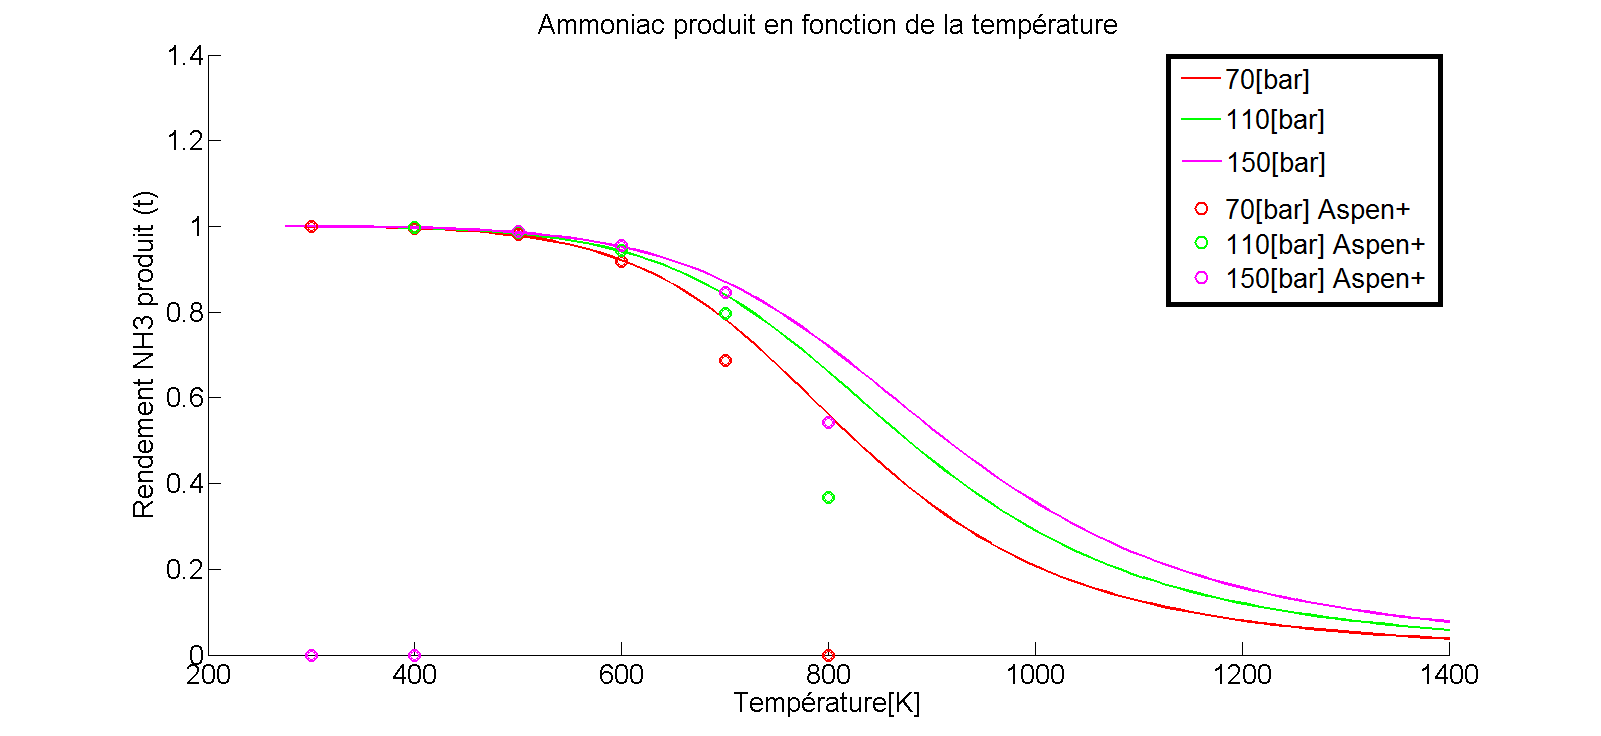
\includegraphics[scale=0.4]{GrapheCompT.png}
 \caption{Rendement en fonction de la température}
 \label{scheme}
\end{figure}

\begin{figure}[ht!]
 \centering
 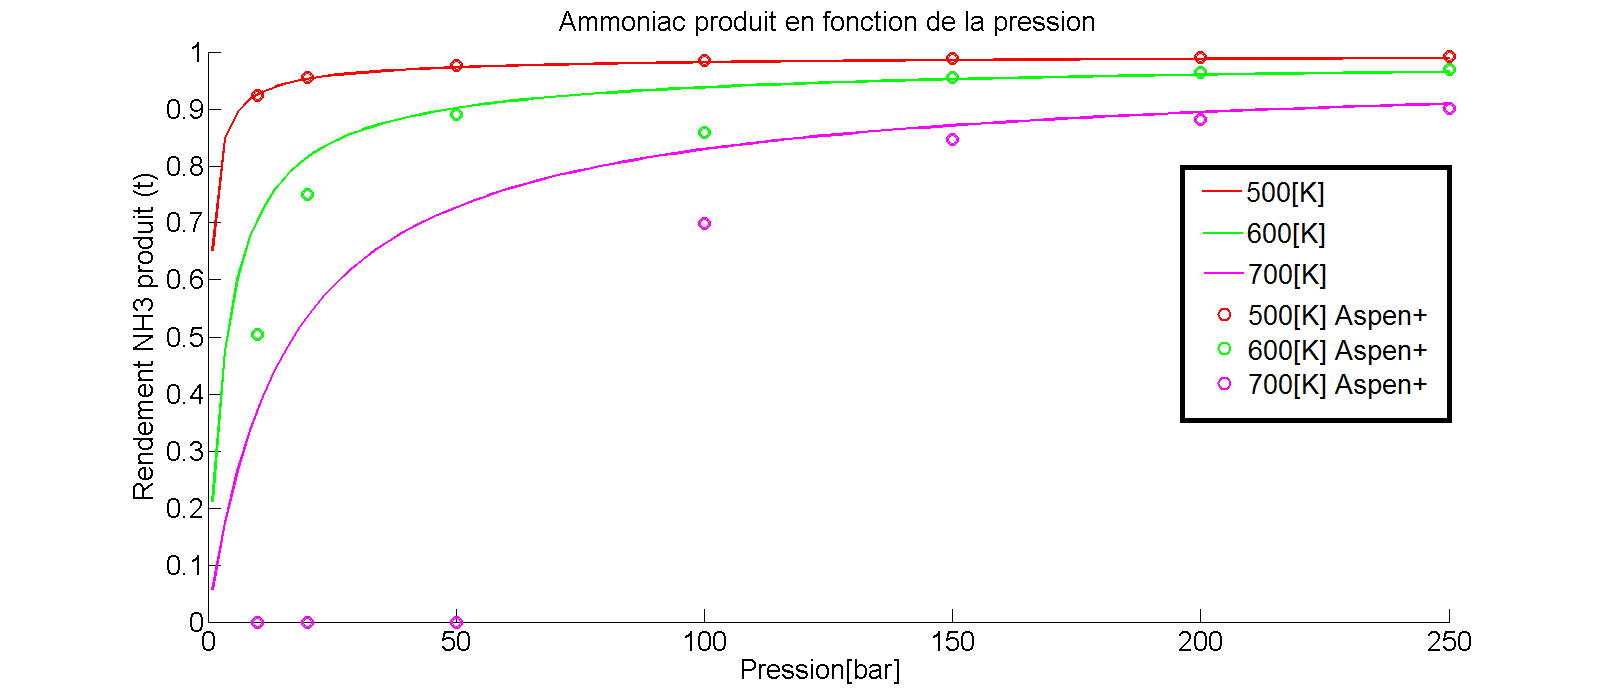
\includegraphics[scale=0.4]{GrapheCompP.png}
 \caption{Rendement en fonction de la pression}
 \label{scheme}
\end{figure}

Dans les deux cas, nous remarquons que l'influence de la température et de la pression font évoluer le rendement dans un même sens: une augmentation de pression et une diminution de la température optimise ce dernier.

Une seconde analyse paramétrique a été réalisée afin d'observer l'influence du taux de purge. Nous nous attendions à avoir une évolution du rendement lorsque celui-ci diminuait. L'analyse a été effectuée pour une pression de \unit{150}{bar}, une température de \unit{500}{\celsius} et pour une production théorique de \unit{1500}{\tonne} Les résultats obtenus sont les suivants:

\begin{figure}[ht!]
 \centering
 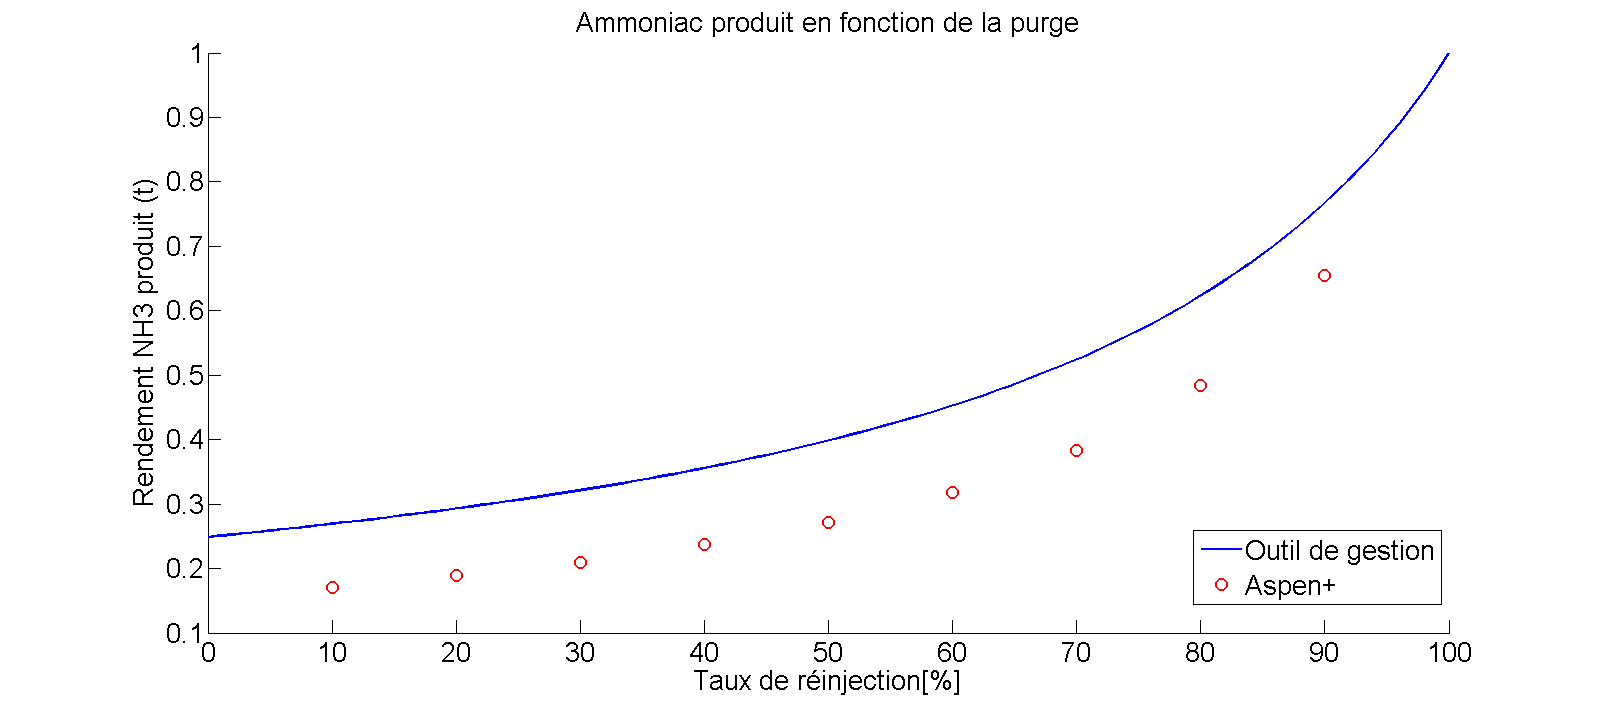
\includegraphics[scale=0.4]{GrapheCompPu.png}
 \caption{Rendement en fonction du taux de purge}
 \label{scheme}
\end{figure}

Comme le montre ce graphique, nous obtenons le résultat attendu. Au plus la taux de purge est élevé, au moins le rendement l'est.

Les différences entre le résultat obtenu avec \textsc{Aspen+} et notre outil de gestion peuvent provenir de plusieurs éléments comme les imprécisions calculatoires de l'un ou l'autre logiciel. Du plus, cela peut aussi être dû au fait que la simulation réalisée avec Aspen+ prenait plus d'éléments en compte que notre outil de gestion, comme la pression présente dans les différents tuyaux et jonctions ainsi que la température au sein de ces derniers. Nous avons fixés ces pressions et température sur base du flowsheet détaillé reçu afin de réaliser la tâche 4. 